\documentclass{article}


\usepackage[spanish]{babel}
\usepackage{gensymb}
\usepackage[letterpaper,top=2cm,bottom=2cm,left=3cm,right=3cm,marginparwidth=1.75cm]{geometry}

% Useful packages
\usepackage{amsmath}
\usepackage{graphicx}
\usepackage[colorlinks=true, allcolors=blue]{hyperref}

\title{Circuito trifásico, practica}
\author{Nehuen Ivanovic Goncalves Da Silva}
\date{}
\begin{document}
\maketitle
\section{Ejercicio 1}
\subsection{a}
Carga conectada en estrella con neutro conectado
\subsection{b}
 es una carga equilibrada
\subsection{c}
Todas las cargas son capacitivas, porque con ese ángulo la corriente adelanta a la tensión, pero no son puras.
\subsection{d}
\[V_F_r=220V\perp0=220\]
\[V_F_s=220V\perp120\circ=-110+j190.56\]
\[V_F_t=220V\perp240\circ=-110-j190.56\]
\subsection{e}
Es una terna de derecha.
\subsection{f}
Las tensiones de linea son:
\[V_L_{s-r}=V_f_s-V_f_r=-110+j190.56-(220)=-330+j190.56\]
\[V_L_{t-s}=V_f_t-V_f_s=-110-j190.56-(-110+j190.56)=-381.12j\]
\[V_L_{r-t}=V_f_r-V_f_t=220-(-110-j190.56)=330+190.56\]

\subsection{g}
\[I_F_r=\frac{V_F_r}{Z_{r-n}}=\frac{220V\perp0}{20\perp-\frac{\pi}{6}}=9.53+5.5j\]
\[I_F_s=\frac{V_F_s}{Z_{s-n}}=\frac{220V\perp\frac{2\pi}{3}}{20\perp-\frac{\pi}{6}}=11A\perp \frac{5\pi}{6}=-9.53+5.5j\]
\[I_F_t=\frac{V_F_t}{Z_{t-n}}=\frac{220V\perp\frac{4\pi}{3}}{20\perp-\frac{\pi}{6}}=11A\perp \frac{7\pi}{6}=0-11j\]

Como es un sistema equilibrado, la corriente que circula por el neutro es nula y las corrientes de fase coincide con las de linea.

\subsection{h}
\begin{equation}
    P_W_r=V_r*I_r*\cos{(-30)}=220*11*\cos{(-30)}=2420\cos{(-30)}
\end{equation}
\begin{equation}
    P_W_s=2420\cos{(-30)}
\end{equation}
\begin{equation}
    P_W_t=2420\cos{(-30)}
\end{equation}
\begin{equation}
    P_{total activa}=P_W_t+P_W_r+P_W_s=3*2420\cos{(-30)}=6287.34W
\end{equation}
\begin{equation}
    P_{total reactiva}=P_W_t+P_W_r+P_W_s=3*2420\sin{(-30)}=-3630VAR
\end{equation}
\begin{equation}
    S_{total}=|I_F_r|*|V_F_r|+|I_F_s|*|V_F_s|+|I_F_t|*|V_F_t|=11A*220V*3=7260VA
\end{equation}
\subsection{i}
Al estar las cargas equilibradas, la corriente y la tensión se mantiene nulas
\subsection{j}
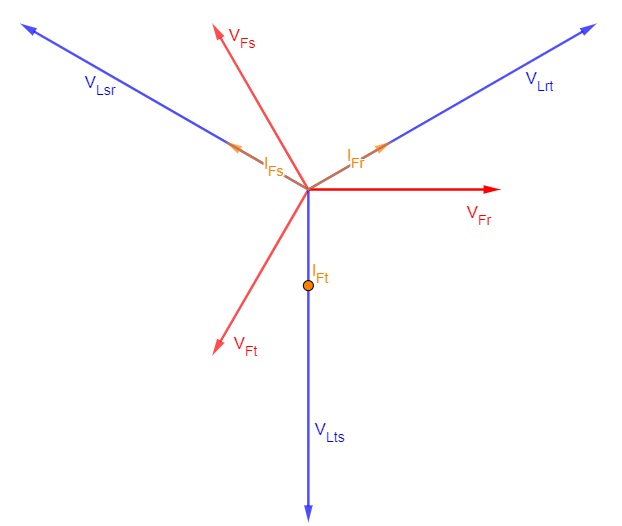
\includegraphics[scale=0.6]{Diagrama_fasorial_1.png}
corrientes escala (10:1)
\section{}
\subsection{a}
El circuito esta conectada como estrella con neutro.
\subsection{b}
El circuito esta desequilibrado
\subsection{c}
$Z_{r-n}$ es una impedancia resistiva.
$Z_{t-n}$ y $Z_{s-n}$ son inductivas.
\subsection{d}
\[V_F_r=220V\perp0=220\]
\[V_F_s=220V\perp120\circ=-110+j190.56\]
\[V_F_t=220V\perp240\circ=-110-j190.56\]
\subsection{e}
\[V_L_{s-r}=-330+j190.56\]
\[V_L_{t-s}=-381.12j\]
\[V_L_{r-t}=330+190.56\]
\subsection{f}
\[I_F_r=\frac{V_F_r}{Z_{r-n}}=\frac{220V\perp0}{6\perp0}=36.67A\]
\[I_F_s=\frac{V_F_s}{Z_{s-n}}=\frac{220V\perp120}{6\perp30\circ}=36.67A\perp90\circ=36.37j\]
\[I_F_t=\frac{V_F_t}{Z_{t-n}}=\frac{220V\perp240}{5\perp45\circ}=44A\perp195\circ=-42.5-11.39j\]
\[I_n=I_F_t+I_F_r+I_F_s=36.67+36.37j-42.5-11.39j=-5.83+24.98j\]
La corrientes de lineas sin iguales a las de fases en este circuito
\subsection{g}
Potencia reactiva:
\[Q_{r}=V_F_{r}\cdot I_F_{r}\cdot\sin(\beta_{r})= 220\cdot 36.67\sin(0)=0VAR\]
\[Q_{s}=V_F_{s}\cdot I_F_{s}\cdot\sin(\beta_{s})=220V \cdot36.67A\sin(30)=4033.7VAR\]
\[Q_{t}=V_F_{t}\cdot I_F_{t}\cdot\sin(\beta_{t})=220V\cdot44A\sin(45)=6844.79VAR\]
\[Q_t=Q_{r}+Q_{s}+Q_{t}=10878.49VAR\]
Potencia Activa:
\[P_{r}=V_F_{r}\cdot I_F_{r}\cdot\cos(\beta_{r})=220\cdot 36.67\cos(0)=8067.4W\]
\[P_{s}=V_F_{s}\cdot I_F_{s}\cdot\cos(\beta_{s})=220V\cdot36.67A\cos(30)=6986.57W\]
\[P_{t}=V_F_{t}\cdot
I_F_{t}\cdot\cos(\beta_{t})=220V\cdot44A\cos(45)=6844.79W\]
\[P_t=P_{r}+P_{s}+P_{t}=21898.76W\]
Potencia aparente:
\[S_{r}=V_F_{s-r}\cdot I_F_{r}\cdot=220\cdot 36.67=8067VA\]
\[S_{s}=V_F_{t-s}\cdot I_F_{s}\cdot=220\cdot 36.67=8067VA\]
\[S_{t}=V_F_{r-t}\cdot I_F_{t}\cdot=220\cdot 44=9680VA\]
\[S_t=P_{r}+S_{s}+S_{t}=25814VA\]
\subsection{h}

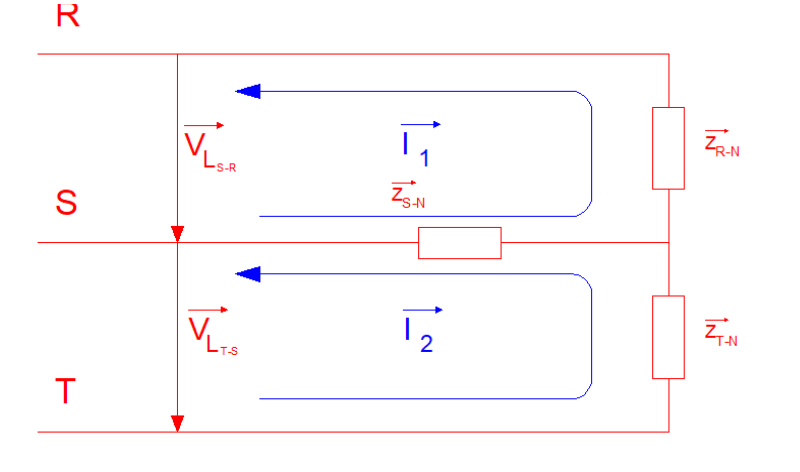
\includegraphics[scale=0.5]{hola.png}
Planteamos las ecuaciones de las mallas.
\[V_{Lsr}-I_1\cdot Z_{s-n}-I_1\cdot Z_{r-n}+I_2\cdot Z_{s-n}=0\]
\[V_{Lts}-I_2\cdot Z_{t-n}-I_2\cdot Z_{s-n}+I_1\cdot Z_{s-n}=0\]
\[V_{Lsr}=I_1(Z{s-n}+Z_{r-n})-I_2\cdot Z_{s-n}\]
\[V_{Lts}=-I_1\cdot Z_{s-n}+I_2(Z_{t-n}+Z_{s-n})\]
Resolvemos plantiando las matrices.
\begin{equation}
\begin{vmatrix}
    Z{s-n}+Z_{r-n} & -Z_{s-n} \\
    -Z_{s-n} & (Z_{t-n}+Z_{s-n})
\end{vmatrix}
\end{equation}

con:
\[Z{s-n}=6\perp30=5.2+3j\]
\[Z{r-n}=6\perp0=6\]
\[Z{t-n}=5\perp45=3.54+j3.54\]
\[V_{Lsr}=-330+j190.56\]
\[V_{Lts}=-381.12j\]
\begin{equation}
\Delta=\begin{vmatrix}
    5.2+3j+6 & -5.2-3j \\
    -5.2-3j & 3.54+j3.54+5.2+3j
\end{vmatrix}=60.23+68.26j=91.04\perp48.58
\end{equation}
\begin{equation}
\Delta I_1=\begin{vmatrix}
    -330+j190.56 & -5.2-3j \\
    -381.12j & 3.54+j3.54+5.2+3j
\end{vmatrix}=-2987.10-2474.53j=3878.93\perp-140.36
\end{equation}
\begin{equation}
\Delta I_2=\begin{vmatrix}
    5.2+3j+6 & -330+j190.56 \\
    -5.2-3j & -381.12j
\end{vmatrix}=-1144.32-4267.63j=4478.35\perp-105.01
\end{equation}
\[I_1=\frac{\Delta I_1}{\Delta}=\frac{3878.93\perp-140.36}{91.04\perp48.58}=42.61\perp-188.94= -42.09+6.62j\]
\[I_2=\frac{\Delta I_2}{\Delta}=\frac{4478.35\perp-105.01}{91.04\perp48.58}=49.19\perp-153.59=−44.06 -21.88j\]
\[I_Fr=-I_1=42.61\perp-8.94=42.09-6.62j\]
\[I_Fs=I_1-I_2=−42.09+6.62j+44.06-21.88j=28.5j+1.97=28.57\perp86.05\]
\[I_Ft=I_2=49.19\perp-153.59=-44.06 -21.88j\]
\[I_{n}=I_r+I_s+I_t=−44.06 -21.88j+28.5j+1.97+42.09-6.62j=0\]

\[V_Zr=I_Fr*Z_{r-n}=42.61\perp-8.94*6\perp=255.66\perp-8.94=252.46-39.71j\]
\[V_Zs=I_Fs*Z_{s-n}=28.57\perp86.05*6\perp30=171.42\perp116.05=-75.28+154.01j\]
\[V_Zt=I_Ft*Z_{t-n}=49.19\perp-153.59*5\perp45=245.95\perp-108.59=-78.31-232.83j\]
\[V_{ON}=V_{Fr}-V_Zr=220-252.46+39.71j=-32.46+39.71j\]
\subsection{i}
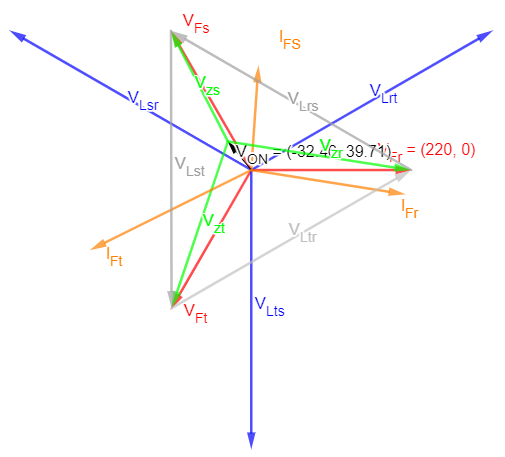
\includegraphics[scale=0.5]{diagrama_fasorial2.png}
Escala para corrientes (5:1)
\section{}
\subsection{a}
Las cargas están conectadas en triangulo
\subsection{b}
Las cargas están desequilibradas
\subsection{c}
$Z_{r-t}$ es resistiva
$Z_{s-r}$ es inductiva pura
$Z_{t-s}$ es inductiva pero no pura
\subsection{d}
\[V_F_r=220V\perp0=220\]
\[V_F_s=220V\perp120\circ=-110+j190.56\]
\[V_F_t=220V\perp240\circ=-110-j190.56\]
\subsection{e}
\[V_L_{s-r}=-330+j190.56=381.04\perp150\]
\[V_L_{t-s}=-381.12j=381.04\perp270\]
\[V_L_{r-t}=330+190.56=381.04\perp30\]
\subsection{f}
\[I_L_{s-r}=\frac{V_L_{s-r}}{Z_{s-r}}=\frac{381.04\perp150}{25\perp90}=15.24\perp60=7.62+13.2j\]
\[I_L_{t-s}=\frac{V_L_{t-s}}{Z_{t-s}}=\frac{381.04\perp270}{15\perp30}=25.4\perp240=-12.7-22j\]
\[I_L_{r-t}=\frac{V_L_{r-t}}{Z_{r-t}}=\frac{381.04\perp30}{20\perp0}=19.05\perp30=16.5+9.53j\]

Corrientes de fase:
\[I_F_r=I_L_{s-r}-I_L_{r-t}=7.62+13.2j-(16.5+9.53j)=3.67j-8.88\]
\[I_F_s=I_L_{t-s}-I_L_{s-r}=-12.7-22j-(7.62+13.2j)=-35.2j-20.32\]
\[I_F_t=I_L_{r-t}-I_L_{t-s}=16.5+9.53j-(-12.7-22j)=31.53j+29.2\]
\[I_n=I_F_t+I_F_r+I_F_s=31.53j+29.2+3.67j-8.88-35.2j-20.32=0\]
\subsection{g}
Potencia reactiva:
\[Q_{s-r}=V_L_{s-r}\cdot I_L_{s-r}\cdot\sin(\beta_{s-r})=381.04\cdot 15.24\sin(90)=5807.2VAR\]
\[Q_{t-s}=V_L_{t-s}\cdot I_L_{t-s}\cdot\sin(\beta_{t-s})=381.04\cdot 25.4\sin(30)=4,838.7VAR\]
\[Q_{r-t}=V_L_{r-t}\cdot I_L_{r-t}\cdot\sin(\beta_{r-t})=381.04\cdot 19.05\sin(0)=0VAR\]
\[Q_t=Q_{s-r}+Q_{t-s}+Q_{r-t}=10645.9VAR\]
Potencia Activa:
\[P_{s-r}=V_L_{s-r}\cdot I_L_{s-r}\cdot\cos(\beta_{s-r})=381.04\cdot 15.24\cos(90)=0W\]
\[P_{t-s}=V_L_{t-s}\cdot I_L_{t-s}\cdot\cos(\beta_{t-s})=381.04\cdot 25.4\cos(30)=8381.75W\]
\[P_{r-t}=V_L_{r-t}\cdot I_L_{r-t}\cdot\cos(\beta_{r-t})=381.04\cdot 19.05\cos(0)=7258.81W\]
\[P_t=P_{s-r}+P_{t-s}+P_{r-t}=15640.56W\]
Potencia aparente:
\[S_{s-r}=V_L_{s-r}\cdot I_L_{s-r}\cdot=381.04\cdot 15.24=5807.05VA\]
\[S_{t-s}=V_L_{t-s}\cdot I_L_{t-s}\cdot=381.04\cdot 25.4=9678.42VA\]
\[S_{r-t}=V_L_{r-t}\cdot I_L_{r-t}\cdot=381.04\cdot 19.05=7258.81VA\]
\[S_t=P_{s-r}+S_{t-s}+S_{r-t}=22744.10VA\]
\subsection{h}
Con el método de los dos Watimetros podemos hallar la Potencia activa total disipada por las cargas, a traves de la suma de las dos lecturas en cada Watimetro.\\
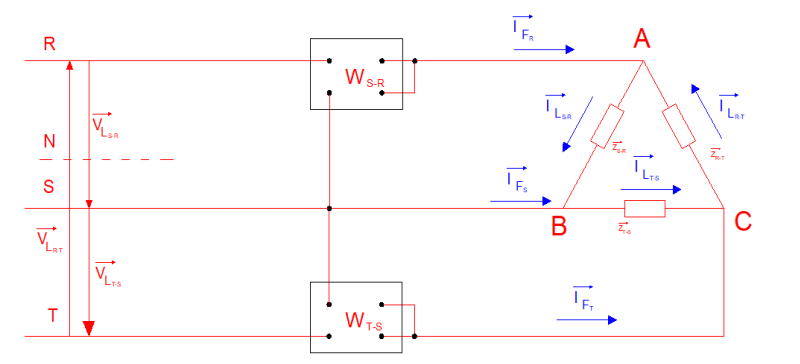
\includegraphics[scale=0.5]{watimetos.png}
\subsection{i}
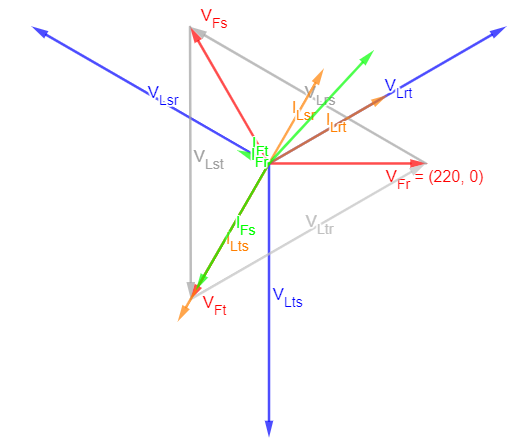
\includegraphics[scale=0.7]{fasores_3.png}
\end{document}